\section{Examples for 2D Reverse Fault with Splay}
\label{sec:example:reverse:2d}

% ----------------------------------------------------------------------
\subsection{Overview}

This suite of examples demonstrates use of a number of features for a
simple two-dimensional model. This example also shows how to produce
a mesh with a somewhat complex geometry. Although the problem geometry
(Figure~\ref{fig:example:reverse:2d:geometry}) includes a simple
planar splay fault intersecting a planar thrust fault, the first 3
steps actually focus on gravitational body forces, reference stresses,
and incompressible elasticity. The fourth example demonstrates the use
of traction boundary conditions to represent a surface load. The
remainder of the examples focus on slip on one or more faults,
including an example of multiple ruptures on a single fault.
To keep the meshing and computation time in these
examples short, we limit our model to a 200 km $\times$ 100 km
domain and we will use a relatively coarse discretization.

\begin{figure}[htbp]
  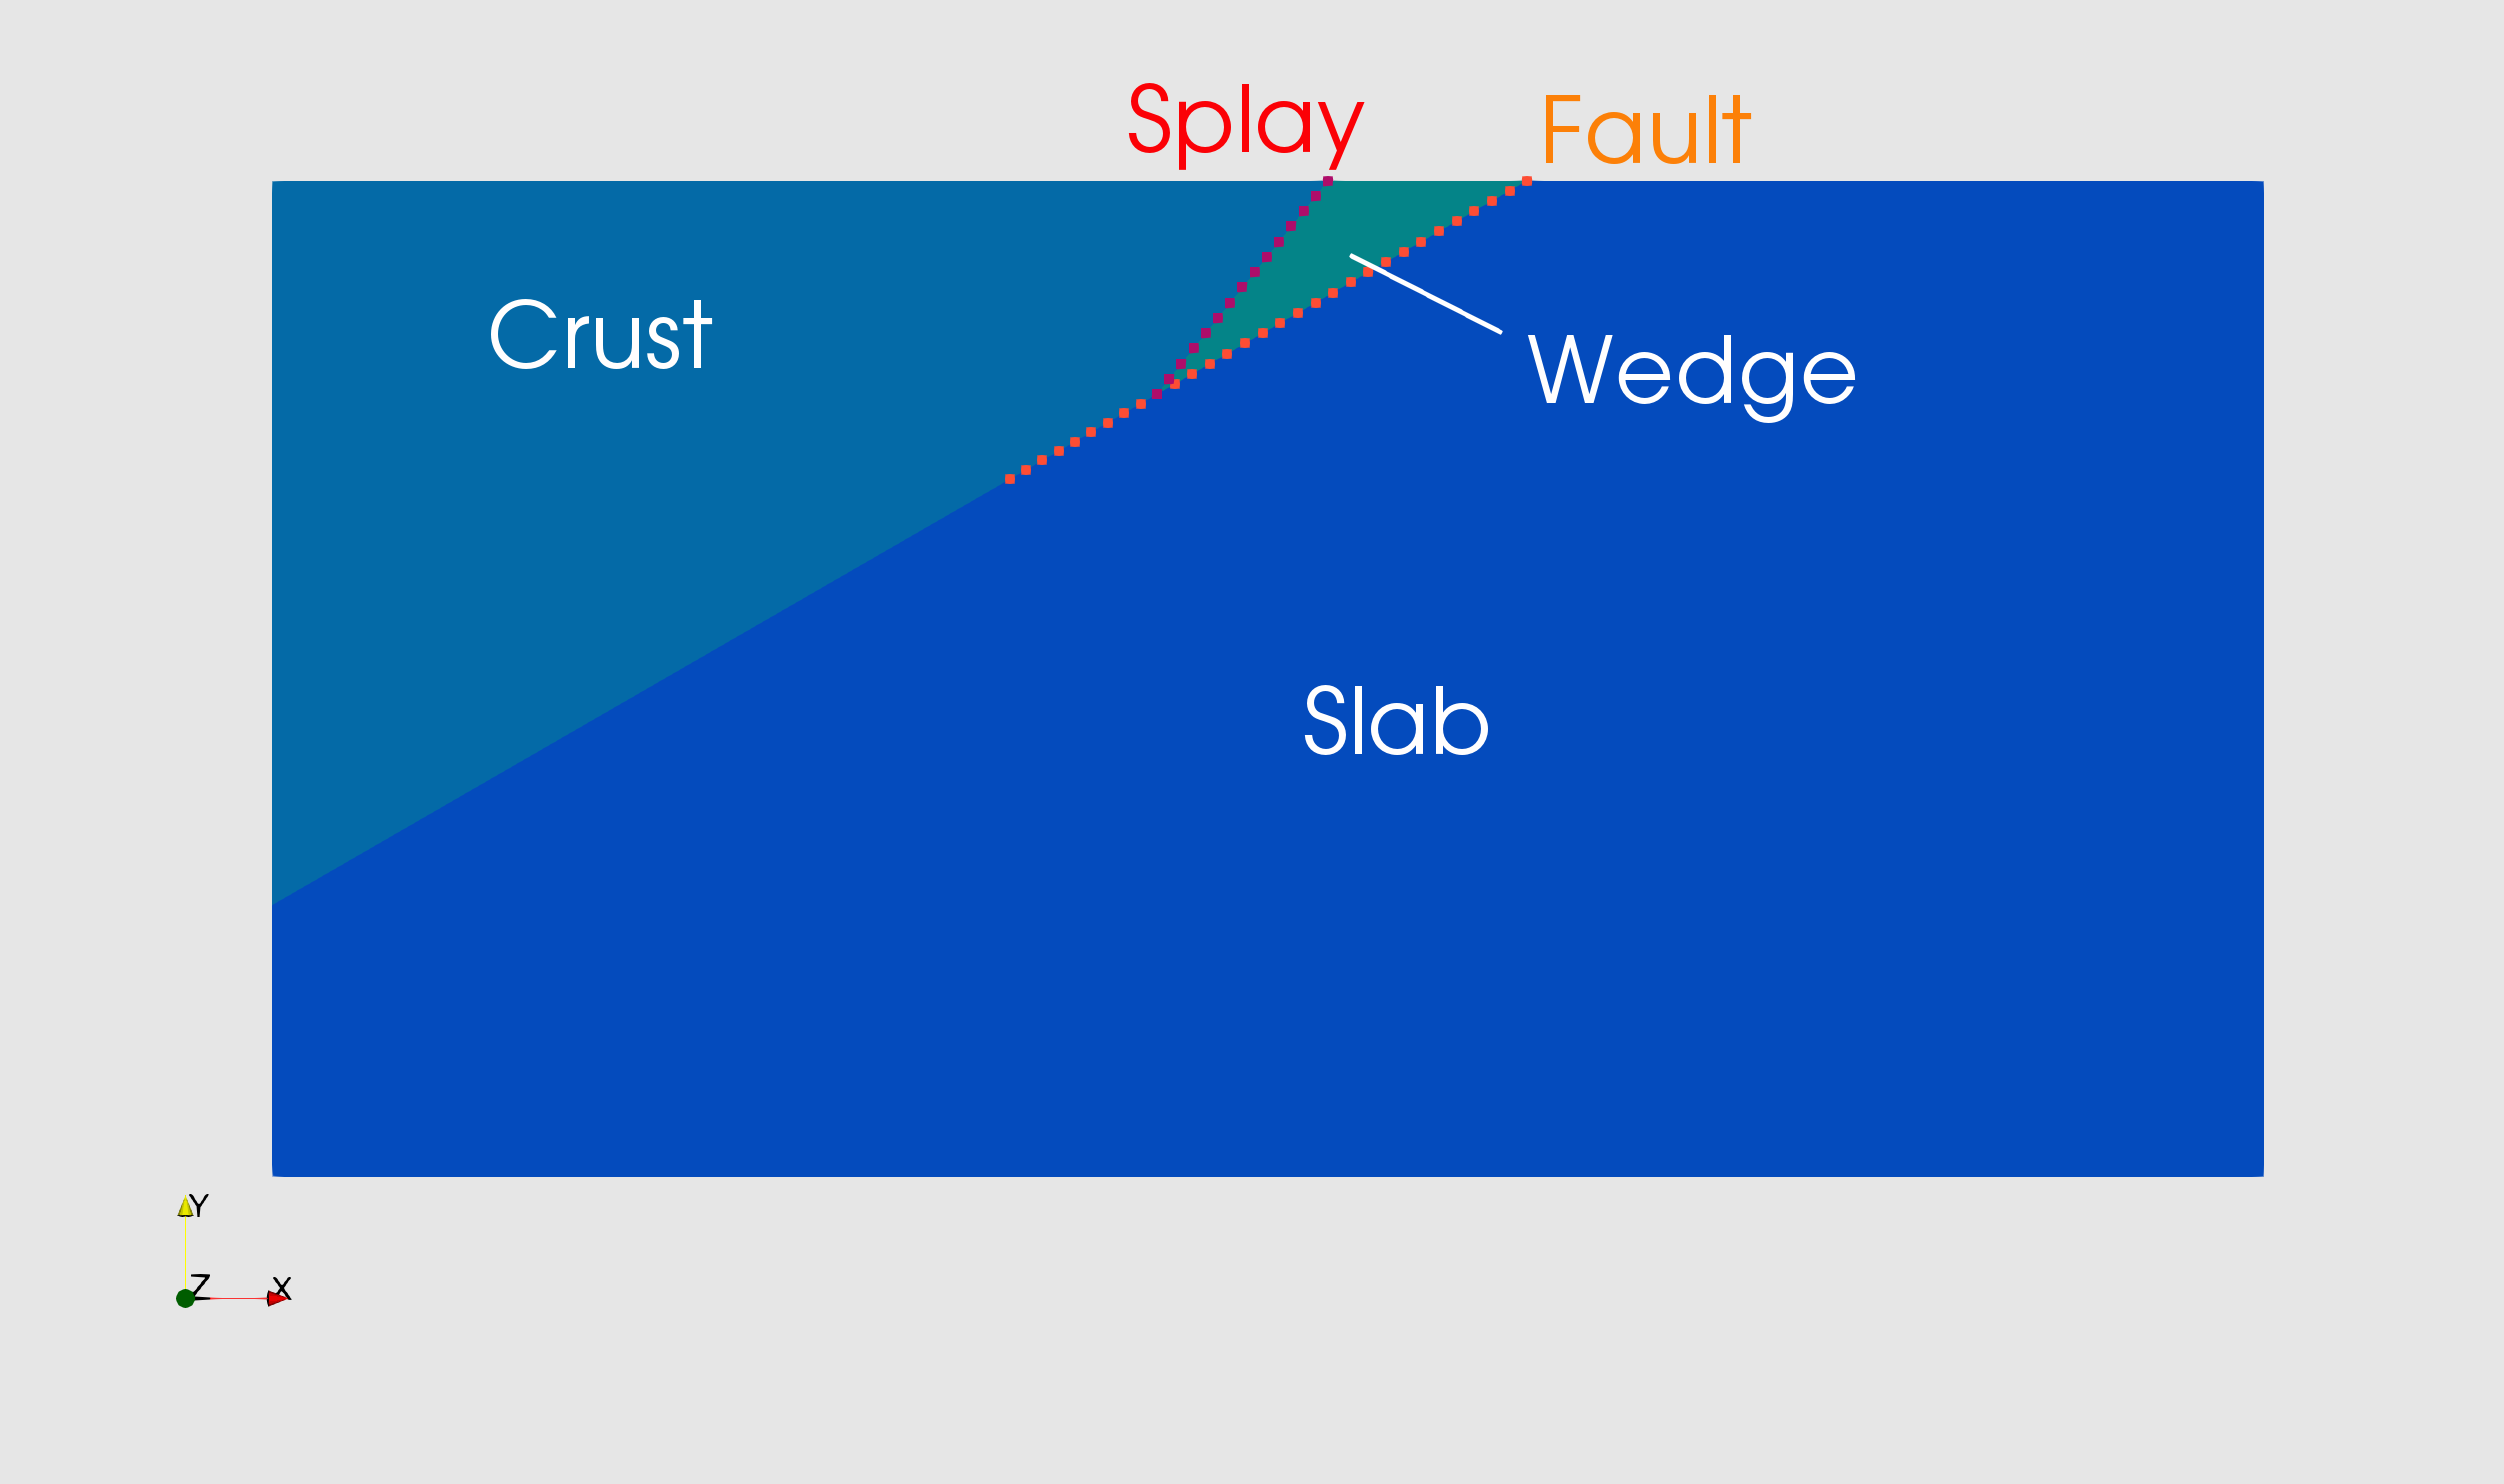
\includegraphics[width=4.5in]{examples/figs/reverse2d_geometry}
  \caption{Geometry used for 2D reverse fault example.}
  \label{fig:example:reverse:2d:geometry}
\end{figure}

Note that although we label the different parts of the mesh as slab,
crust, and wedge, the actual thrust fault only extends 60 km downdip,
and we do not provide bottom boundaries for the crust and slab.
The files associated with this suite of examples are contained in the
directory \filename{examples/2d/reverse}. This directory contains
several files:
\begin{description}
\item[\filename{*.jou}] Files used to construct the finite-element mesh using
  CUBIT/Trelis.
\item[\filename{*.spatialdb}] Files associated with the spatial databases.
\item[\filename{viz}] Directory containing ParaView
  Python scripts and other files for visualizing results.
\item[\filename{output}] Directory containing simulation
  output. It is created automatically when running the
  simulations.
\item[\filename{README.md}] README file containing a brief description
  of the various examples.
\end{description}


% ----------------------------------------------------------------------
\subsection{Features Illustrated}

Table~\ref{tab:example:reverse:2d:features} lists the features
discussed in each of these 2-D reverse fault examples. With the
intent of illustrating features used in research simulations, we use
HDF5 output and we make extensive use the most efficient
implementations of spatial databases (UniformDB and ZeroDB). We
also use ParaView Python scripts for visualizing the output. These
scripts can be run within the ParaView GUI or outside the ParaView
GUI, although the interaction is limited to rotating, translating, and
zooming when run outside the ParaView GUI.

% \begin{table}[htbp]
%   \caption{PyLith features covered in the suite of 2-D reverse fault examples.}
%   \label{tab:example:reverse:2d:features}
%   \input{examples/2d_reverse_features}
% \end{table}

% ----------------------------------------------------------------------
\subsection{Generating the Finite-Element Mesh}

We use CUBIT/Trelis to generate the finite-element mesh. Due to the
small size of these 2D meshes, we include them in the PyLith source
and binary distributions. If you do not have CUBIT/Trelis, you can
use the provided meshes.

Mesh generation is controlled from either \filename{mesh\_tri.jou}
(triangular meshes) or \filename{mesh\_quad.jou} (quadrilateral
meshes). In addition to creating the desired meshes, these scripts
call the following additional journal files:
\begin{description}
\item[\filename{geometry.jou}] Journal file to create the 2D geometry.
\item[\filename{gradient.jou}] Journal file to assign sizing
  information for the mesh.
\item[\filename{createbc.jou}] Journal file to define material blocks
  and nodesets for boundary conditions.
\end{description}

The first step is to create the geometry. This consists of creating a
brick, extracting a midsurface from it, and then splitting the
remaining surface with an extended fault and a splay surface. The
surfaces, curves, and important vertices are then assigned names that
are then used when setting up mesh sizing information and defining
blocks and nodesets.

\important{We use IDless journaling in CUBIT/Trelis. This allows us to
  reference objects in a manner that should be independent of the
  version of CUBIT/Trelis that is being used. In the journal files,
  the original command used is typically commented out, and the
  following command is the equivalent IDless command.}

Once the geometry has been generated, we then set sizing information
using both a user-defined sizing function as well as the CUBIT/Trelis
curve and surface bias schemes. Using this sizing information, an
initial mesh is generated, and then one iteration of smoothing is
performed to improve the cell quality. Finally, blocks are defined for
the three materials in the problem, and nodesets are also defined for
the fault and splay surfaces.

\important{In addition to providing nodesets for the fault and splay,
  it is also important to provide nodesets defining the buried edges
  of these two surfaces. In 2D, this will consist of a single vertex
  for each surface. This information is required by PyLith to form the
  corresponding cohesive cells defining fault surfaces.}

Once you have run either the \filename{mesh\_tri.jou} or
\filename{mesh\_quad.jou}journal file to construct the geometry and
generate the mesh, you will have a corresponding Exodus-II file
(\filename{mesh\_tri.exo} or \filename{mesh\_quad.exo}). These are
NetCDF files, and they can be loaded into ParaView. This can be done
by either running ParaView and loading the file, or using the script
provided in the viz directory. For example, if ParaView is in your
path, you can run the following command:
\begin{shell}
  paraview --script=viz/plot_mesh.py
\end{shell}
This will open ParaView, load the mesh, and produce views of both the
mesh (with fault nodeset) and the mesh quality.

\subsection{Organization of Simulation Parameters}
\label{sec:example:reverse:2d:organization}

PyLith automatically reads in \filename{pylithapp.cfg} from the
current directory, if it exists. As a result, we generally put all
parameters common to a set of examples in this file to avoid
duplicating parameters across multiple files. Because we often use a
single mesh for multiple simulations in a directory, we place all
parameters related to our mesh and identifying the materials in our
mesh in \filename{pylithapp.cfg}. We assign the bulk constitutive
model and its parameters to each material in other files, because we
generally vary those across the simulations. In general, we place roller
boundary conditions (Dirichlet boundary conditions constraining the
degrees of freedom perpendicular to the boundary) on the lateral and
bottom boundaries, so we include those in \filename{pylithapp.cfg}. In
some simulations we will overwrite the values for parameters will
values specific to a given example. We also do the same thing for
materials, since most of the examples use the default linear isotropic
material.  This file is also a convenient
place to put basic solver parameters and to turn on Pyre journals for
displaying informational messages during a run.journalling debugging
flags.

% End of file
